\section{Appendix}
\subsection{Ablation Details}

Here, we present detailed qualitative and quantitative results from our ablation study comparing our approach against closely related baselines. We first evaluated replacing the KAN with a standard MLP. Additionally, we experimented with incorporating material tokens or features, similar to scaffolded Gaussian Splats; however, the performance was inferior to that of a straightforward MLP. We also attempted to use spherical Gaussians for the view-dependent representation, but this approach yielded suboptimal results. These quantitative comparisons are summarized in Tab.~\ref{tab:combined-ablation-baselines}.

Furthermore, we provide qualitative visualizations that decompose the outputs of our method. Specifically, our rendering function consists of three components: multiple environment maps for self-reflection, a KAN for specular reflection, and a GMM for diffuse lighting. We visualize the distinct contributions of each of these lighting components. To isolate the effects of the 2D GMM, Fig.~\ref{fig:abl_qualitative} compares our method against a 2DGS baseline exhibiting depth-fighting (with spherical harmonics set to zero). Finally, Tab.~\ref{tab:shiny_perscene} details a per-scene comparison against reported state-of-the-art results on the Shiny-Blender dataset; these methods reconstruct their own geometry rather than being given ours, so, following Table~\ref{tab:main}, they are shown as context rather than ranked.

% Auto-generated ablation tables (8 = 2 datasets x 4 variants)
% metrics: PSNR (dB, higher better), SSIM (higher), LPIPS (lower)
% Auto-generated ablation tables (8 = 2 datasets x 4 variants)
% metrics: PSNR (dB, higher better), SSIM (higher), LPIPS (lower)
\begin{table}[t]
  \centering
  \caption{Ablation comparisons across all datasets and scenes. Ranking
  (\colorbox{green!25}{\textbf{1st}}, \colorbox{orange!25}{2nd}, \colorbox{yellow!25}{3rd}) is
  restricted to Ours, DNR, and 2DGS$^{*}$, the fixed-mesh methods that share our input mesh
  (following Table~\ref{tab:main}); the ablation-variant columns are not ranked, since they trace
  an internal progression rather than a competing baseline.}
  \label{tab:combined-ablation-baselines}
  \resizebox{\linewidth}{!}{
  \begin{tabular}{llccccccc}
    \toprule
    \multirow{2}{*}{Dataset} & \multirow{2}{*}{Scene} & \multicolumn{5}{c}{Ablation Variants} & \multicolumn{2}{c}{Fixed-mesh baselines} \\
    \cmidrule(lr){3-7} \cmidrule(lr){8-9}
    & & MLP+SG+M Token & MLP + M Token & MLP & 1-Env MLP & Ours & DNR & 2DGS$^{*}$ \\
    \midrule
    \multicolumn{9}{c}{\textbf{PSNR$\uparrow$}} \\
    \midrule
    \multirow{9}{*}{\rotatebox{90}{{NeRF-Synthetic}}}
    & Chair     & 33.43 & 31.30 & 33.22 & 33.45 & \cellcolor{orange!25} 33.00 & \cellcolor{yellow!25} 31.91 & \cellcolor{green!25} \textbf{33.63} \\
    & Drums     & 27.16 & 26.98 & 26.97 & 27.42 & \cellcolor{green!25} \textbf{27.81} & \cellcolor{yellow!25} 25.11 & \cellcolor{orange!25} 25.90 \\
    & Ficus     & 32.45 & 32.43 & 32.48 & 32.66 & \cellcolor{yellow!25} 32.94 & \cellcolor{green!25} \textbf{35.42} & \cellcolor{orange!25} 33.73 \\
    & Hotdog    & 37.15 & 36.74 & 37.03 & 37.13 & \cellcolor{green!25} \textbf{37.60} & \cellcolor{orange!25} 37.43 & \cellcolor{yellow!25} 36.53 \\
    & Lego      & 35.47 & 34.98 & 35.45 & 35.54 & \cellcolor{green!25} \textbf{36.14} & \cellcolor{yellow!25} 34.11 & \cellcolor{orange!25} 34.46 \\
    & Materials & 32.24 & 32.48 & 32.25 & 32.26 & \cellcolor{green!25} \textbf{34.58} & \cellcolor{orange!25} 28.83 & \cellcolor{yellow!25} 27.34 \\
    & Mic       & 35.12 & 35.64 & 35.09 & 35.41 & \cellcolor{green!25} \textbf{36.66} & \cellcolor{yellow!25} 34.89 & \cellcolor{orange!25} 35.96 \\
    & Ship      & 30.28 & 30.56 & 30.27 & 30.66 & \cellcolor{green!25} \textbf{31.18} & \cellcolor{yellow!25} 28.41 & \cellcolor{orange!25} 31.02 \\
    \cmidrule{2-9}
    & \textbf{Mean} & 32.91 & 32.64 & 32.84 & 33.07 & \cellcolor{green!25} \textbf{33.74} & \cellcolor{yellow!25} 32.01 & \cellcolor{orange!25} 32.32 \\
    \midrule
    \multirow{7}{*}{\rotatebox{90}{Shiny-Blender}}
    & Ball      & 40.32 & 43.90 & 39.74 & 40.38 & \cellcolor{green!25} \textbf{45.01} & \cellcolor{orange!25} 21.83 & \cellcolor{yellow!25} 20.99 \\
    & Car       & 28.07 & 29.49 & 28.18 & 29.50 & \cellcolor{green!25} \textbf{33.75} & \cellcolor{yellow!25} 21.11 & \cellcolor{orange!25} 26.41 \\
    & Coffee    & 33.47 & 34.28 & 33.28 & 32.85 & \cellcolor{green!25} \textbf{35.33} & \cellcolor{yellow!25} 31.04 & \cellcolor{orange!25} 32.26 \\
    & Helmet    & 34.19 & 35.82 & 34.27 & 34.16 & \cellcolor{green!25} \textbf{37.94} & \cellcolor{orange!25} 26.82 & \cellcolor{yellow!25} 26.23 \\
    & Teapot    & 44.72 & 46.96 & 44.18 & 44.40 & \cellcolor{green!25} \textbf{47.45} & \cellcolor{orange!25} 43.60 & \cellcolor{yellow!25} 40.75 \\
    & Toaster   & 24.66 & 23.15 & 24.25 & 24.92 & \cellcolor{green!25} \textbf{28.76} & \cellcolor{orange!25} 20.58 & \cellcolor{yellow!25} 19.55 \\
    \cmidrule{2-9}
    & \textbf{Mean} & 34.24 & 35.60 & 33.98 & 34.37 & \cellcolor{green!25} \textbf{38.04} & \cellcolor{yellow!25} 27.50 & \cellcolor{orange!25} 27.70 \\

    \midrule
    \multicolumn{9}{c}{\textbf{SSIM$\uparrow$}} \\
    \midrule
    \multirow{9}{*}{\rotatebox{90}{{NeRF-Synthetic}}}
    & Chair     & 0.9797 & 0.9682 & 0.9790 & 0.9797 & \cellcolor{orange!25} 0.9767 & \cellcolor{yellow!25} 0.9747 & \cellcolor{green!25} \textbf{0.9808} \\
    & Drums     & 0.9558 & 0.9583 & 0.9545 & 0.9572 & \cellcolor{green!25} \textbf{0.9629} & \cellcolor{yellow!25} 0.9427 & \cellcolor{orange!25} 0.9502 \\
    & Ficus     & 0.9772 & 0.9777 & 0.9773 & 0.9782 & \cellcolor{yellow!25} 0.9800 & \cellcolor{green!25} \textbf{0.9848} & \cellcolor{orange!25} 0.9820 \\
    & Hotdog    & 0.9849 & 0.9848 & 0.9845 & 0.9848 & \cellcolor{green!25} \textbf{0.9869} & \cellcolor{orange!25} 0.9859 & \cellcolor{yellow!25} 0.9826 \\
    & Lego      & 0.9812 & 0.9808 & 0.9812 & 0.9814 & \cellcolor{green!25} \textbf{0.9836} & \cellcolor{yellow!25} 0.9764 & \cellcolor{orange!25} 0.9765 \\
    & Materials & 0.9670 & 0.9733 & 0.9671 & 0.9671 & \cellcolor{green!25} \textbf{0.9812} & \cellcolor{orange!25} 0.9523 & \cellcolor{yellow!25} 0.9193 \\
    & Mic       & 0.9884 & 0.9896 & 0.9883 & 0.9894 & \cellcolor{green!25} \textbf{0.9918} & \cellcolor{yellow!25} 0.9861 & \cellcolor{orange!25} 0.9892 \\
    & Ship      & 0.8941 & 0.9091 & 0.8943 & 0.9023 & \cellcolor{green!25} \textbf{0.9145} & \cellcolor{yellow!25} 0.8688 & \cellcolor{orange!25} 0.8995 \\
    \cmidrule{2-9}
    & \textbf{Mean} & 0.9660 & 0.9677 & 0.9658 & 0.9675 & \cellcolor{green!25} \textbf{0.9722} & \cellcolor{yellow!25} 0.9590 & \cellcolor{orange!25} 0.9600 \\
    \midrule
    \multirow{7}{*}{\rotatebox{90}{Shiny-Blender}}
    & Ball      & 0.9847 & 0.9935 & 0.9837 & 0.9848 & \cellcolor{green!25} \textbf{0.9945} & \cellcolor{orange!25} 0.9075 & \cellcolor{yellow!25} 0.8860 \\
    & Car       & 0.9320 & 0.9453 & 0.9322 & 0.9384 & \cellcolor{green!25} \textbf{0.9763} & \cellcolor{yellow!25} 0.8835 & \cellcolor{orange!25} 0.9207 \\
    & Coffee    & 0.9669 & 0.9754 & 0.9660 & 0.9682 & \cellcolor{green!25} \textbf{0.9777} & \cellcolor{yellow!25} 0.9662 & \cellcolor{orange!25} 0.9672 \\
    & Helmet    & 0.9759 & 0.9868 & 0.9763 & 0.9760 & \cellcolor{green!25} \textbf{0.9902} & \cellcolor{orange!25} 0.9525 & \cellcolor{yellow!25} 0.9403 \\
    & Teapot    & 0.9963 & 0.9979 & 0.9959 & 0.9960 & \cellcolor{green!25} \textbf{0.9983} & \cellcolor{orange!25} 0.9961 & \cellcolor{yellow!25} 0.9942 \\
    & Toaster   & 0.9113 & 0.9262 & 0.9037 & 0.9165 & \cellcolor{green!25} \textbf{0.9607} & \cellcolor{orange!25} 0.8812 & \cellcolor{yellow!25} 0.8736 \\
    \cmidrule{2-9}
    & \textbf{Mean} & 0.9612 & 0.9708 & 0.9596 & 0.9633 & \cellcolor{green!25} \textbf{0.9830} & \cellcolor{orange!25} 0.9312 & \cellcolor{yellow!25} 0.9303 \\

    \midrule
    \multicolumn{9}{c}{\textbf{LPIPS$\downarrow$}} \\
    \midrule
    \multirow{9}{*}{\rotatebox{90}{{NeRF-Synthetic}}}
    & Chair     & 0.0167 & 0.0255 & 0.0176 & 0.0168 & \cellcolor{yellow!25} 0.0197 & \cellcolor{orange!25} 0.0186 & \cellcolor{green!25} \textbf{0.0119} \\
    & Drums     & 0.0388 & 0.0416 & 0.0402 & 0.0376 & \cellcolor{green!25} \textbf{0.0361} & \cellcolor{yellow!25} 0.0547 & \cellcolor{orange!25} 0.0451 \\
    & Ficus     & 0.0307 & 0.0302 & 0.0306 & 0.0302 & \cellcolor{yellow!25} 0.0278 & \cellcolor{green!25} \textbf{0.0109} & \cellcolor{orange!25} 0.0126 \\
    & Hotdog    & 0.0144 & 0.0151 & 0.0150 & 0.0146 & \cellcolor{yellow!25} 0.0130 & \cellcolor{green!25} \textbf{0.0110} & \cellcolor{orange!25} 0.0127 \\
    & Lego      & 0.0112 & 0.0119 & 0.0112 & 0.0108 & \cellcolor{green!25} \textbf{0.0095} & \cellcolor{yellow!25} 0.0153 & \cellcolor{orange!25} 0.0146 \\
    & Materials & 0.0245 & 0.0213 & 0.0245 & 0.0243 & \cellcolor{green!25} \textbf{0.0138} & \cellcolor{orange!25} 0.0446 & \cellcolor{yellow!25} 0.0532 \\
    & Mic       & 0.0179 & 0.0131 & 0.0179 & 0.0165 & \cellcolor{orange!25} 0.0097 & \cellcolor{yellow!25} 0.0189 & \cellcolor{green!25} \textbf{0.0091} \\
    & Ship      & 0.0758 & 0.0793 & 0.0760 & 0.0728 & \cellcolor{green!25} \textbf{0.0691} & \cellcolor{yellow!25} 0.1669 & \cellcolor{orange!25} 0.0751 \\
    \cmidrule{2-9}
    & \textbf{Mean} & 0.0288 & 0.0297 & 0.0291 & 0.0279 & \cellcolor{green!25} \textbf{0.0248} & \cellcolor{yellow!25} 0.0426 & \cellcolor{orange!25} 0.0293 \\
    \midrule
    \multirow{7}{*}{\rotatebox{90}{Shiny-Blender}}
    & Ball      & 0.0496 & 0.0248 & 0.0540 & 0.0490 & \cellcolor{green!25} \textbf{0.0224} & \cellcolor{yellow!25} 0.1848 & \cellcolor{orange!25} 0.1651 \\
    & Car       & 0.0432 & 0.0340 & 0.0428 & 0.0387 & \cellcolor{green!25} \textbf{0.0154} & \cellcolor{yellow!25} 0.1120 & \cellcolor{orange!25} 0.0418 \\
    & Coffee    & 0.0506 & 0.0470 & 0.0525 & 0.0504 & \cellcolor{green!25} \textbf{0.0427} & \cellcolor{yellow!25} 0.0681 & \cellcolor{orange!25} 0.0442 \\
    & Helmet    & 0.0350 & 0.0181 & 0.0347 & 0.0346 & \cellcolor{green!25} \textbf{0.0130} & \cellcolor{orange!25} 0.0617 & \cellcolor{yellow!25} 0.0724 \\
    & Teapot    & 0.0080 & 0.0049 & 0.0085 & 0.0085 & \cellcolor{green!25} \textbf{0.0039} & \cellcolor{orange!25} 0.0052 & \cellcolor{yellow!25} 0.0083 \\
    & Toaster   & 0.1201 & 0.0975 & 0.1324 & 0.1148 & \cellcolor{green!25} \textbf{0.0455} & \cellcolor{yellow!25} 0.1503 & \cellcolor{orange!25} 0.1380 \\
    \cmidrule{2-9}
    & \textbf{Mean} & 0.0511 & 0.0377 & 0.0541 & 0.0493 & \cellcolor{green!25} \textbf{0.0238} & \cellcolor{yellow!25} 0.0970 & \cellcolor{orange!25} 0.0783 \\
    \bottomrule
  \end{tabular}
  }
\end{table}

\begin{table}[t]
  \centering
  \caption{Per-scene comparison on Shiny-Blender against reported results for methods that
  reconstruct their own geometry. Following Table~\ref{tab:main}, these are not given our input
  mesh, so they are shown as context rather than ranked against \textbf{Ours}, which is bolded
  for reference only.}
  \label{tab:shiny_perscene}
  \resizebox{\linewidth}{!}{
  \begin{tabular}{lccccccc}
    \toprule
    & \multicolumn{7}{c}{Shiny-Blender} \\
    & Car & Ball & Helmet & Teapot & Toaster & Coffee & Avg. \\
    \midrule
    \multicolumn{8}{c}{PSNR$\uparrow$} \\
    \midrule
    Ref-NeRF~\citep{refnerf} &  30.41 & 29.14 & 29.92 & 45.19 & 25.29 & 33.99 & 32.32 \\
    NeRO~\citep{nero} & 25.53 & 30.26 & 29.20 & 38.70 & 26.46 & 28.89 & 29.84 \\
    ENVIDR~\citep{envidr} & 28.46 & 38.89 & 32.73 & 41.59 & 26.11 & 29.48 & 32.88 \\
    3DGS~\citep{3DGS} & 27.24 & 27.69 & 28.32 & 45.68 & 20.99 & 32.32 & 30.37 \\
    GaussianShader~\citep{gaussianShader} & 27.51 & 29.02 & 28.73 & 43.05 & 22.86 & 31.34 & 30.42 \\
    3iGS~\citep{3igs} & 27.52 & 26.82 & 28.08 & 46.05 & 22.71 & 32.64 & 30.64 \\
    3DGS-DR~\citep{3dgsDR} & 30.43 & 33.44 & 31.49 & 47.00 & 26.69 & 34.61 & 33.94 \\
    RefGS~\citep{refgs}                & 30.94 & 36.10 & 33.40 & 46.69 & 27.28 & 34.38 & 34.80 \\
    \midrule
    \textbf{Ours}     &  \textbf{33.75} & \textbf{45.01} & \textbf{37.94} & \textbf{47.45} & \textbf{28.76} & \textbf{35.33} & \textbf{38.04} \\
    \midrule
    \multicolumn{8}{c}{SSIM$\uparrow$} \\
    \midrule
    Ref-NeRF~\citep{refnerf} & 0.949 & 0.956 & 0.955 & 0.995 & 0.910 & 0.972 & 0.956 \\
    NeRO~\citep{nero} & 0.949 & 0.974 & 0.971 & 0.995 & 0.929 & 0.956 & 0.962 \\
    ENVIDR~\citep{envidr} & 0.961 & 0.991 & 0.980 & 0.996 & 0.939 & 0.949 & 0.969 \\
    3DGS~\citep{3DGS} & 0.930 & 0.937 & 0.951 & 0.996 & 0.895 & 0.971 & 0.947 \\
    GaussianShader~\citep{gaussianShader} & 0.930 & 0.954 & 0.955 & 0.996 & 0.900 & 0.969 & 0.951 \\
    3iGS~\citep{3igs} & 0.930 & 0.933 & 0.951 & 0.996 & 0.909 & 0.972 & 0.948 \\
    3DGS-DR~\citep{3dgsDR} & 0.962 & 0.979 & 0.971 & 0.997 & 0.942 & 0.976 & 0.971 \\
    RefGS~\citep{refgs}               & 0.961 & 0.981 & 0.975 & 0.997 & 0.942 & 0.973 & 0.973 \\
    \midrule
    \textbf{Ours}            & \textbf{0.9763} & \textbf{0.9945} & \textbf{0.9902} & \textbf{0.9983} & \textbf{0.9607} & \textbf{0.9777} & \textbf{0.9830} \\
    \midrule
    \multicolumn{8}{c}{LPIPS$\downarrow$} \\
    \midrule
    Ref-NeRF~\citep{refnerf} & 0.051 & 0.307 & 0.087 & 0.013 & 0.118 & 0.082 & 0.110 \\
    NeRO~\citep{nero} & 0.074 & 0.094 & 0.050 & 0.012 & 0.089 & 0.110 & 0.072 \\
    ENVIDR~\citep{envidr} & 0.049 & 0.067 & 0.051 & 0.011 & 0.116 & 0.139 & 0.072 \\
    3DGS~\citep{3DGS} & 0.047 & 0.161 & 0.079 & 0.007 & 0.126 & 0.078 & 0.083 \\
    GaussianShader~\citep{gaussianShader} & 0.045 & 0.148 & 0.088 & 0.012 & 0.111 & 0.085 & 0.082 \\
    3iGS~\citep{3igs} & 0.045 & 0.166 & 0.073 & 0.006 & 0.098 & 0.077 & 0.077 \\
    3DGS-DR~\citep{3dgsDR} & 0.034 & 0.104 & 0.050 & 0.006 & 0.083 & 0.076 & 0.059 \\
    RefGS~\citep{refgs}                & 0.034 & 0.098 & 0.045 & 0.006 & 0.070 & 0.082 & 0.056 \\
    \midrule
    \textbf{Ours}     & \textbf{0.0154} & \textbf{0.0224} & \textbf{0.0130} & \textbf{0.0039} & \textbf{0.0455} & \textbf{0.0427} & \textbf{0.0238} \\
    \bottomrule
  \end{tabular}
  }
\end{table}



\begin{figure}
    \centering
    \includegraphics[width=\linewidth]{figs/ablation.pdf}
    \caption{From left to right: 2DGS baseline, 2D GMM for diffuse light, KAN with one environment map, KAN with multiple environment maps, and ground truth. We highlight that our multi-environment setting successfully approximates the self-reflection effects on concave objects in toaster. For convex-objects, since there is nearly no self-reflection, the visual results seems highly aligned}
    \label{fig:abl_qualitative}
\end{figure}

\subsection{Mesh Refinement Through the Anchoring}
\label{app:refinement}
Because each disk center is a barycentric combination of its face's vertices
(Eq.~\eqref{eq:center}), the anchoring is linear in the mesh, $\mathbf{X}=\mathbf{B}\mathbf{V}$, and
photometric gradients reach the vertices. We use this to refine an imperfect input mesh (here, one
extracted from Ref-GS's unconstrained Gaussians), as a demonstration of the property rather than as
a new refinement method: the photometric gradient is taken at the disk centers, evaluated at the
ray--disk intersection, and pulled back to the vertices through the anchoring, similar in spirit to
the mesh-anchored refinement of SuGaR~\citep{sugar} and OMeGa~\citep{omega}; connectivity is fixed.

\paragraph{Setup.} We start from the Ref-GS~\citep{refgs} mesh (TSDF fusion and marching cubes,
then simplification and hole filling), warm up the appearance model on it for 625 optimizer steps,
and freeze the KAN shader and environment maps. We then alternate 300 cycles of a geometry step
(8 training views, one vertex update restricted to the vertex normal, smoothed to $2.5\sigma$ and
capped at $0.5\sigma$ per cycle, $\sigma$ the disk radius) and an appearance step (40 steps on the
disks, mesh fixed). The optional prior is an area-weighted normal-consistency term pulling each face
normal toward the input's shading normals, weighted at half the photometric gradient's norm.
Geometry is scored against the ground-truth Blender models. Normals are scored by mean angular
error against the ground-truth normal maps of the 200 test views. For position, we use the standard
DTU metrics~\citep{dtu}, but report only accuracy (Acc.), the mean distance from points on the
refined mesh to the nearest ground-truth surface visible from the test cameras (lower is better).
Following Ref-NeuS~\citep{ref-neus}, we omit completeness, which is dominated by regions missing
from the input mesh that a fixed-connectivity refinement cannot fill.

\paragraph{Results.} Table~\ref{tab:refine_improve} summarizes the effect of refinement on the
input mesh, and Table~\ref{tab:refine_decomp} separates the two signals.
The prior alone reorients faces toward the smooth shading normals, giving the lowest face-normal
error, but it does not use the images and moves the surface away from the ground truth (accuracy
worsens from $5.83$ to $6.18$). The photometric gradient alone is not enough either: without the
prior, face normals degrade ($7.20^\circ \rightarrow 18.58^\circ$). Together they give the best
vertex-normal error ($6.31^\circ \rightarrow 5.41^\circ$) and accuracy ($5.83 \rightarrow 5.49$).
Figure~\ref{fig:mesh_ringing} shows the effect of refinement on high-frequency surface artifacts
left by the extraction: the fine noise on \emph{teapot} and the concentric marching-cubes ringing
on \emph{helmet} are both smoothed away.

\paragraph{Limitations.} The refinement adjusts an existing surface and cannot recover absent
geometry, starts from a short warm-up rather than a fully trained model, and is not compared
against full reconstruction pipelines such as OMeGa or Ref-NeuS, which also change topology or
reconstruct geometry from scratch.

\begin{table}[t]
\centering
\small
\begin{minipage}[t]{0.40\textwidth}
\centering
\caption{\textbf{Effect of refinement on the input mesh} (means over the six Shiny-Blender scenes),
without $\rightarrow$ with refinement (photometric + normal). Improvement is the relative reduction in
error. Metrics as in Table~\ref{tab:refine_decomp}.}
\label{tab:refine_improve}
\setlength{\tabcolsep}{4pt}
\begin{tabular}{@{}lcc@{}}
\toprule
& w/o $\rightarrow$ w/ & Improvement \\
\midrule
$\mathrm{MAE}_{\mathbf{n}_f}$ ($^\circ$)$\downarrow$ & $7.20 \rightarrow 5.88$ & $+18.3\%$ \\
$\mathrm{MAE}_{\mathbf{n}_v}$ ($^\circ$)$\downarrow$ & $6.31 \rightarrow 5.41$ & $+14.2\%$ \\
Acc.\ ($\times10^{-3}$)$\downarrow$         & $5.83 \rightarrow 5.49$ & $+5.8\%$  \\
\bottomrule
\end{tabular}
\end{minipage}
\hfill
\begin{minipage}[t]{0.56\textwidth}
\centering
\caption{\textbf{Where the refinement gain comes from} (means over the six Shiny-Blender scenes,
lower is better; angular errors in degrees, Acc.\ $\times10^{-3}$). Rows name the terms
optimized: the photometric loss, the normal-consistency prior, or both. Per-scene values in
Table~\ref{tab:refine_perscene}.}
\label{tab:refine_decomp}
\setlength{\tabcolsep}{4pt}
\begin{tabular}{@{}lccc@{}}
\toprule
& $\mathrm{MAE}_{\mathbf{n}_f}\downarrow$ & $\mathrm{MAE}_{\mathbf{n}_v}\downarrow$ & Acc.$\downarrow$ \\
\midrule
Input mesh & 7.20 & 6.31 & 5.83 \\
\midrule
Normal only & \textbf{5.55} & 5.88 & 6.18 \\
Photometric only & 18.58 & 6.53 & 6.11 \\
Photometric + normal & 5.88 & \textbf{5.41} & \textbf{5.49} \\
\bottomrule
\end{tabular}
\end{minipage}
\end{table}

\begin{table}[t]
\centering
\footnotesize
\setlength{\tabcolsep}{3pt}
\caption{\textbf{Per-scene refinement results}, same arms and metrics as
Table~\ref{tab:refine_decomp}. Avg.\ averages the per-scene values. \colorbox{green!25}{\textbf{1st}}, \colorbox{orange!25}{2nd}, and \colorbox{yellow!25}{3rd} best per column are highlighted.}
\label{tab:refine_perscene}
\begin{tabular}{@{}lccccccc@{}}
\toprule
& Helmet & Teapot & Toaster & Coffee & Car & Ball & Avg. \\
\midrule
\multicolumn{8}{c}{MAE$_{\mathbf{n}_f}$ ($^\circ$)$\downarrow$} \\
\midrule
Input mesh & \cellcolor{yellow!25} 4.48 & \cellcolor{yellow!25} 7.25 & \cellcolor{yellow!25} 9.40 & \cellcolor{yellow!25} 9.02 & \cellcolor{yellow!25} 9.81 & \cellcolor{yellow!25} 3.21 & \cellcolor{yellow!25} 7.20 \\
Prior only & \cellcolor{green!25} \textbf{1.98} & \cellcolor{orange!25} 4.99 & \cellcolor{orange!25} 8.45 & \cellcolor{orange!25} 8.85 & \cellcolor{green!25} \textbf{8.41} & \cellcolor{green!25} \textbf{0.62} & \cellcolor{green!25} \textbf{5.55} \\
Ours (image only) & 21.42 & 13.16 & 21.51 & 16.31 & 17.53 & 21.54 & 18.58 \\
Ours (image + prior) & \cellcolor{orange!25} 2.41 & \cellcolor{green!25} \textbf{4.71} & \cellcolor{green!25} \textbf{7.85} & \cellcolor{green!25} \textbf{8.21} & \cellcolor{orange!25} 9.09 & \cellcolor{orange!25} 3.01 & \cellcolor{orange!25} 5.88 \\
\midrule
\multicolumn{8}{c}{MAE$_{\mathbf{n}_v}$ ($^\circ$)$\downarrow$} \\
\midrule
Input mesh & 2.77 & 6.69 & \cellcolor{orange!25} 9.02 & \cellcolor{yellow!25} 10.02 & \cellcolor{yellow!25} 8.69 & \cellcolor{yellow!25} 0.64 & \cellcolor{yellow!25} 6.31 \\
Prior only & \cellcolor{orange!25} 2.61 & \cellcolor{orange!25} 5.52 & \cellcolor{yellow!25} 9.08 & \cellcolor{orange!25} 9.08 & \cellcolor{orange!25} 8.40 & \cellcolor{orange!25} 0.58 & \cellcolor{orange!25} 5.88 \\
Ours (image only) & \cellcolor{yellow!25} 2.69 & \cellcolor{yellow!25} 6.44 & 9.69 & 10.35 & 9.34 & 0.67 & 6.53 \\
Ours (image + prior) & \cellcolor{green!25} \textbf{2.48} & \cellcolor{green!25} \textbf{4.89} & \cellcolor{green!25} \textbf{8.23} & \cellcolor{green!25} \textbf{8.32} & \cellcolor{green!25} \textbf{7.96} & \cellcolor{green!25} \textbf{0.57} & \cellcolor{green!25} \textbf{5.41} \\
\midrule
\multicolumn{8}{c}{Acc.\ ($\times10^{-3}$)$\downarrow$} \\
\midrule
Input mesh & \cellcolor{orange!25} 4.40 & \cellcolor{orange!25} 4.25 & \cellcolor{orange!25} 7.93 & \cellcolor{yellow!25} 9.34 & \cellcolor{yellow!25} 4.06 & \cellcolor{orange!25} 4.97 & \cellcolor{orange!25} 5.83 \\
Prior only & 4.74 & 4.58 & \cellcolor{yellow!25} 8.13 & 9.75 & 4.61 & \cellcolor{yellow!25} 5.28 & 6.18 \\
Ours (image only) & \cellcolor{yellow!25} 4.63 & \cellcolor{green!25} \textbf{4.23} & 9.09 & \cellcolor{orange!25} 8.80 & \cellcolor{green!25} \textbf{3.99} & 5.93 & \cellcolor{yellow!25} 6.11 \\
Ours (image + prior) & \cellcolor{green!25} \textbf{3.56} & \cellcolor{yellow!25} 4.30 & \cellcolor{green!25} \textbf{7.60} & \cellcolor{green!25} \textbf{8.72} & \cellcolor{orange!25} 4.02 & \cellcolor{green!25} \textbf{4.72} & \cellcolor{green!25} \textbf{5.49} \\
\bottomrule
\end{tabular}
\end{table}


\begin{figure}
    \centering
    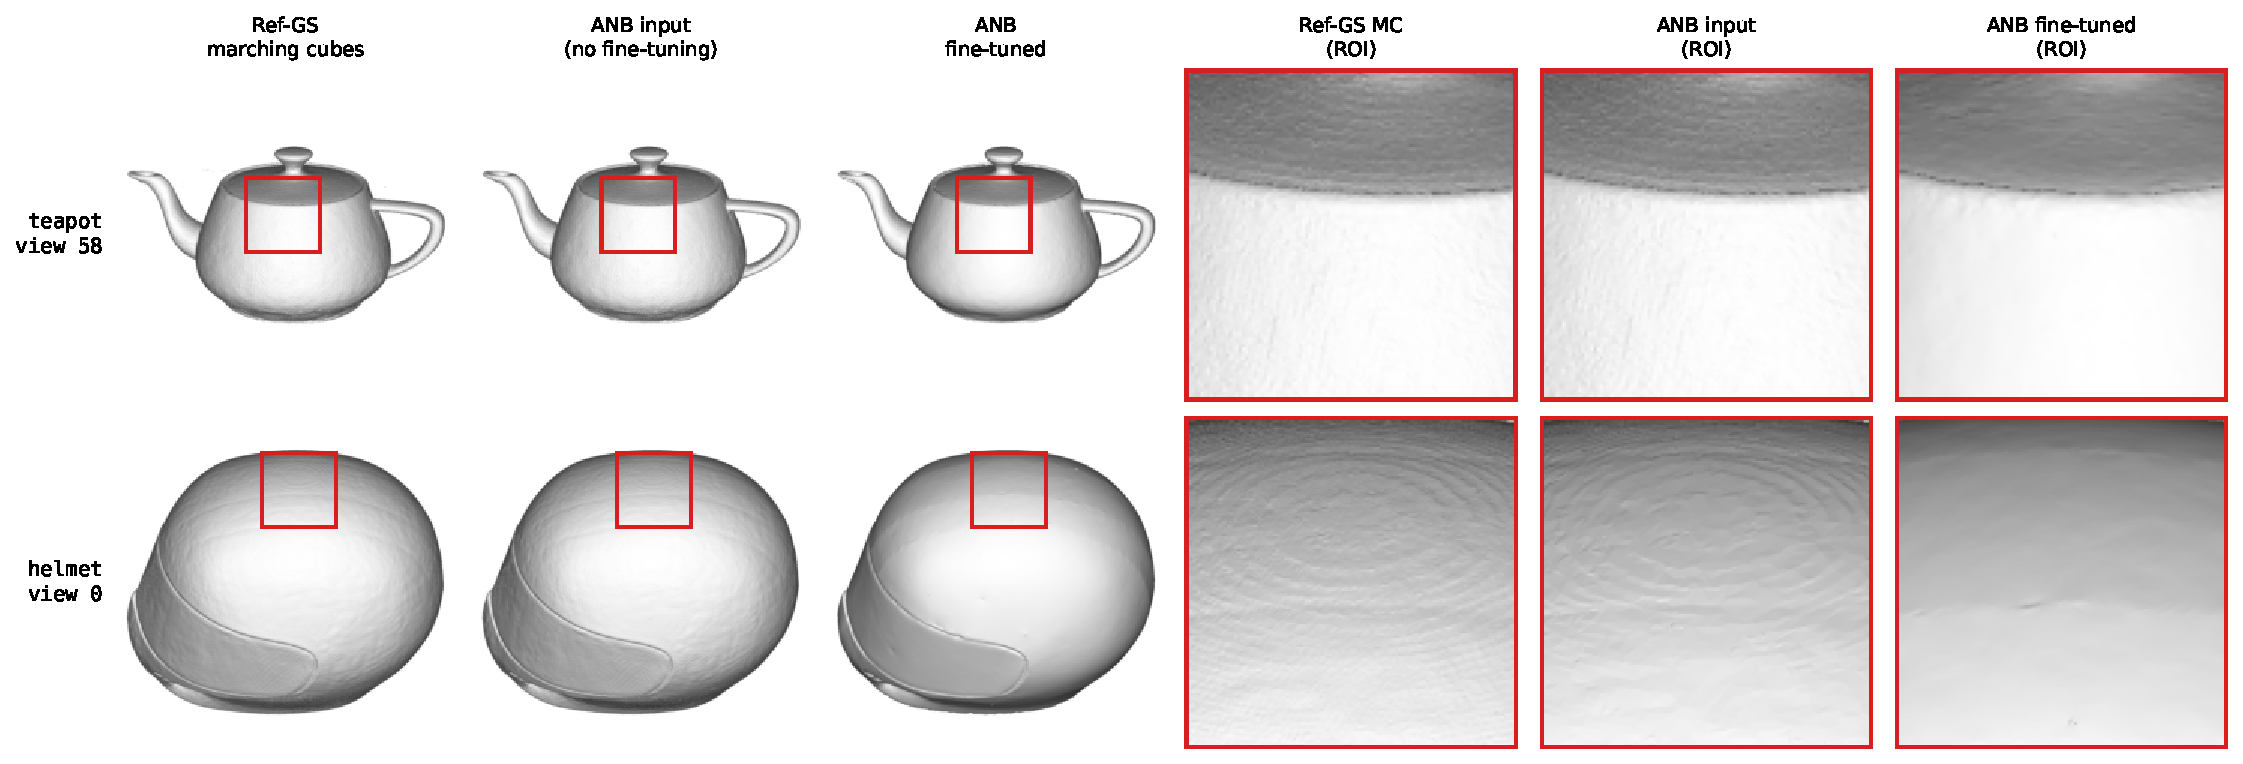
\includegraphics[width=\linewidth]{figs/mesh_ringing.pdf}
    \caption{\textbf{Effect of refinement on high-frequency surface artifacts.} Rows: \emph{teapot}
    and \emph{helmet}. Left two columns: the mesh before (input mesh) and after refinement, region of
    interest boxed in red; right two columns: the boxed region magnified. Refinement removes the
    fine noise on \emph{teapot} and the concentric ringing left by marching-cubes extraction on
    \emph{helmet}.}
    \label{fig:mesh_ringing}
\end{figure}

\begin{figure}
    \centering
    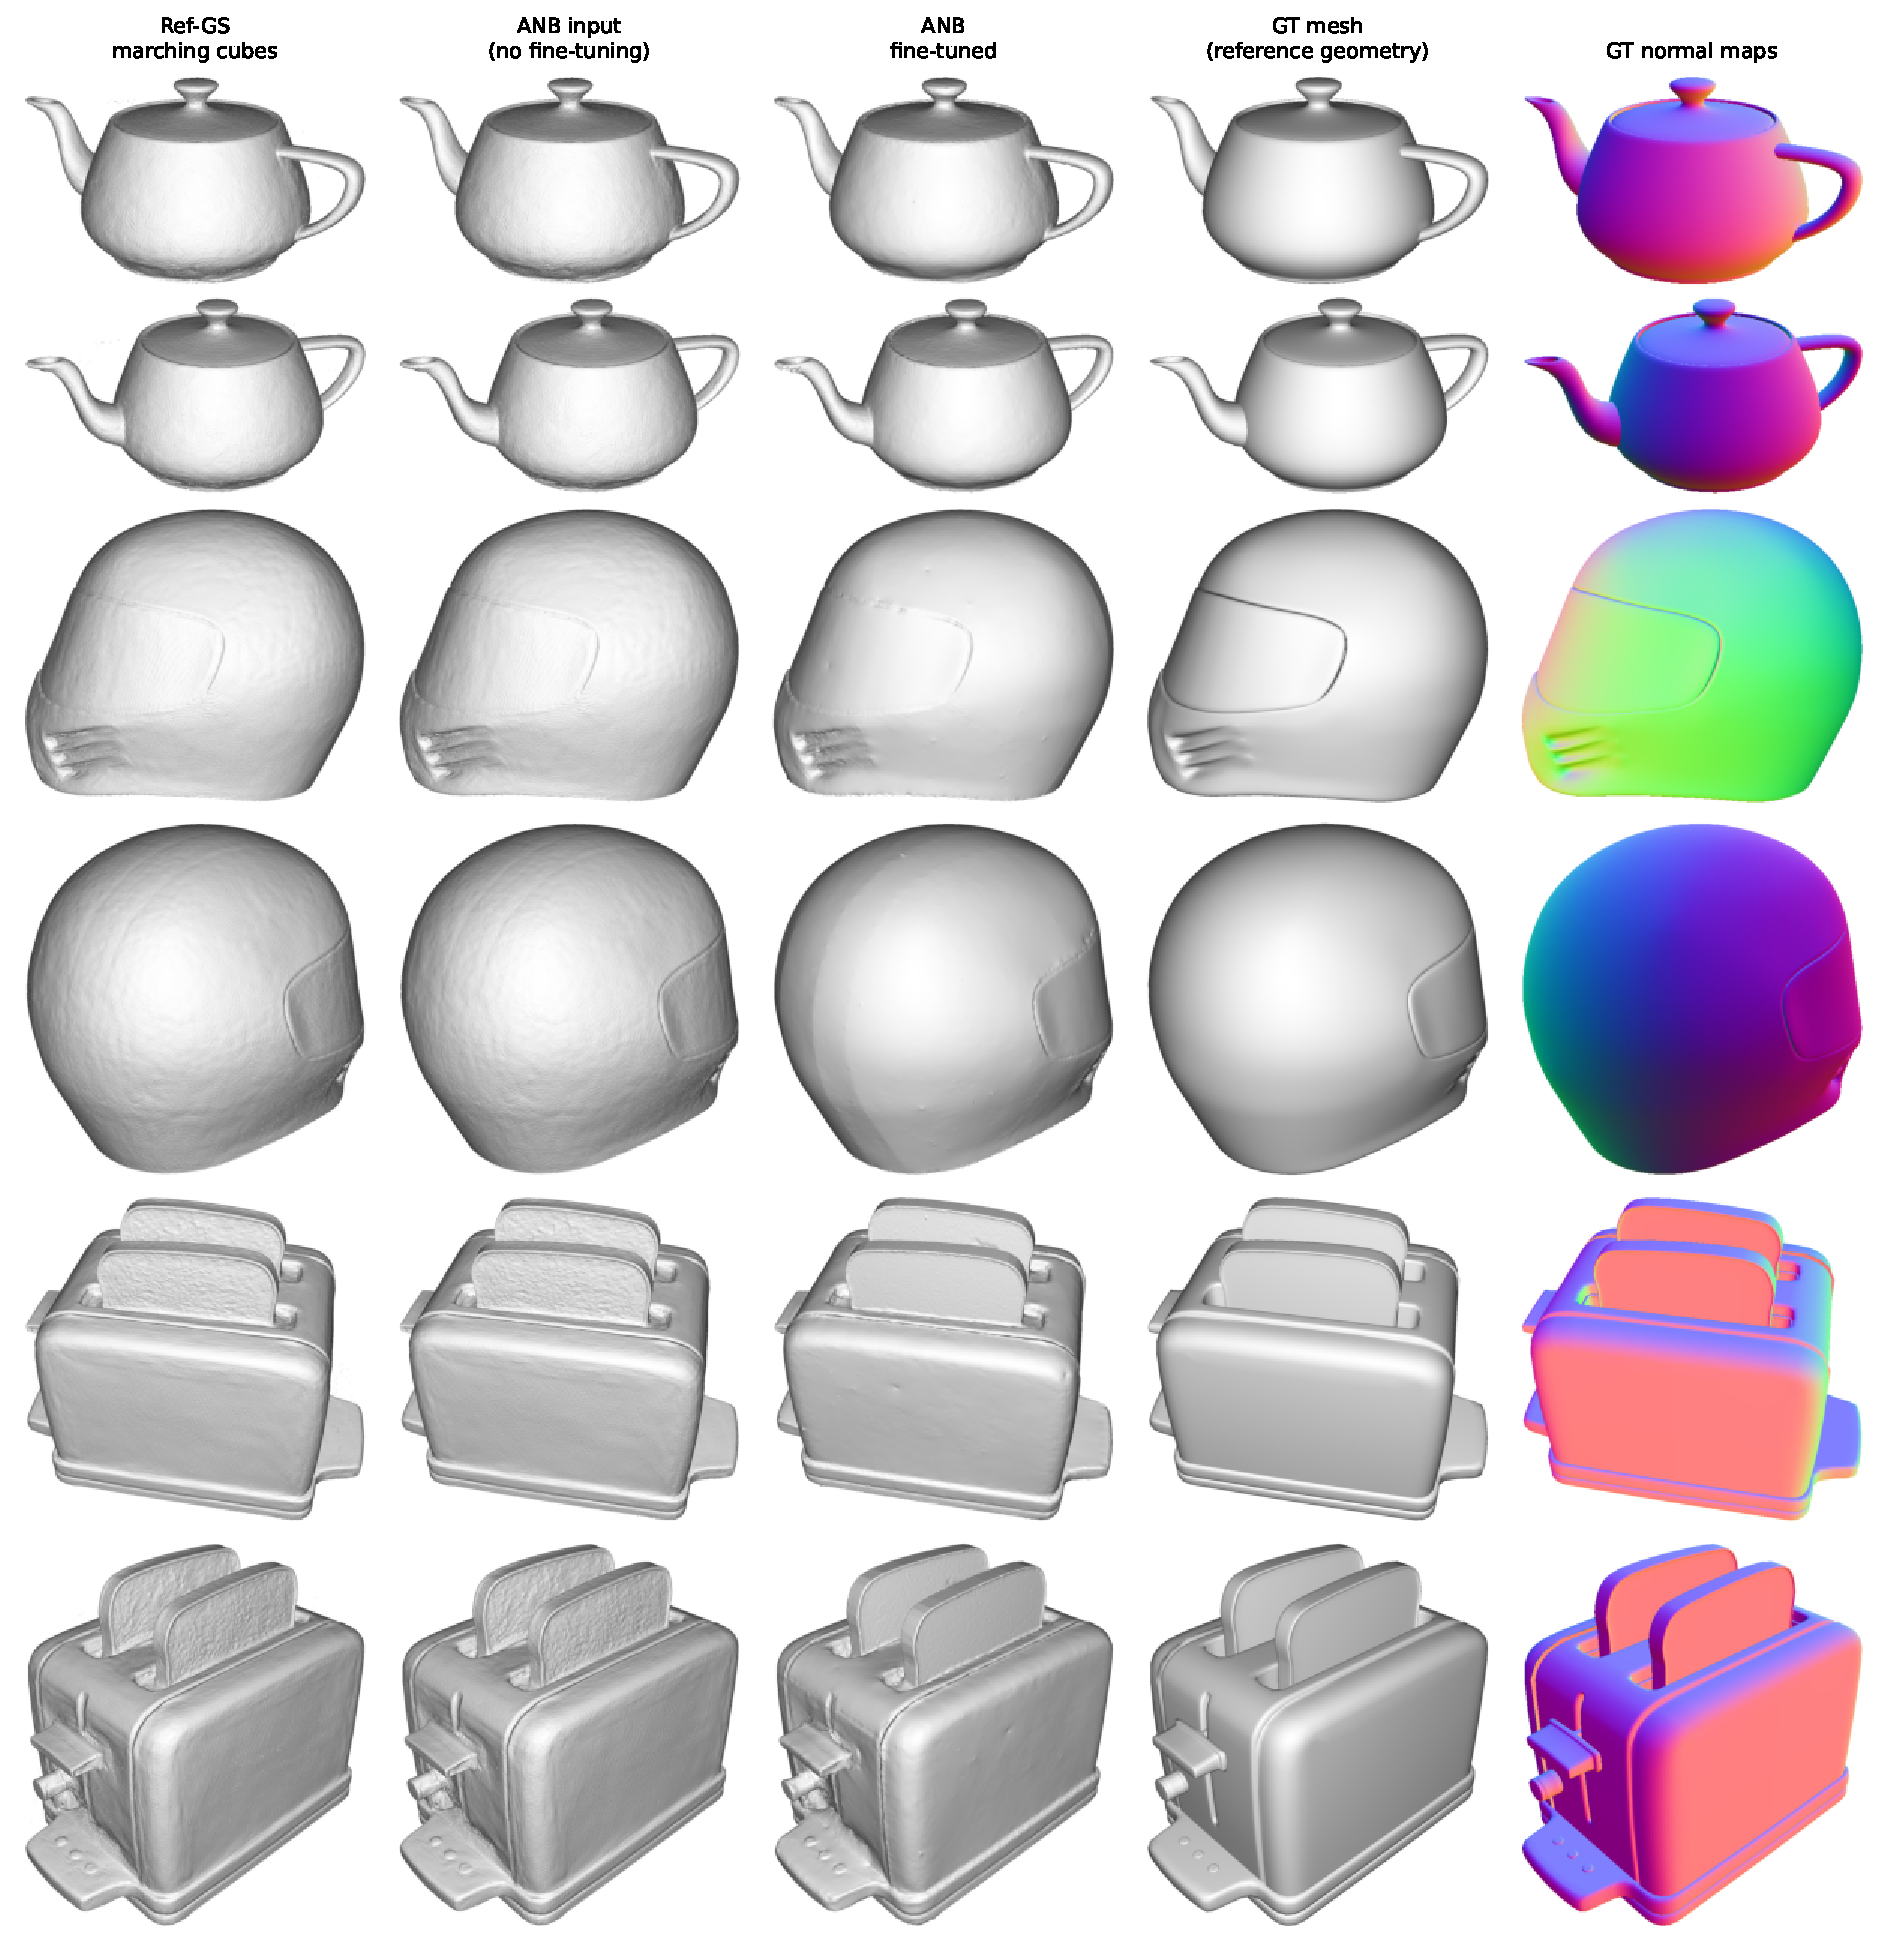
\includegraphics[width=\linewidth]{figs/mesh_qual.pdf}
    \caption{\textbf{Mesh refinement results.} Each row is one held-out test view, two each of \emph{teapot}, \emph{helmet} and \emph{toaster}. \emph{Columns 1--3} follow one mesh through our pipeline and are flat-shaded so that surface defects stay visible: (1) the mesh Ref-GS extracts by TSDF fusion and marching cubes; (2) that mesh after simplification and hole filling, which is the input to refinement; (3) the same mesh after refinement. Columns 1 and 2 differ only by simplification, so the change from column 2 to column 3 is due to refinement alone. \emph{Columns 4--5} are for reference only: the ground-truth mesh (smooth-shaded) and the ground-truth normal map for the same view.}
    \label{fig:mesh_qual}
\end{figure}

\subsection{Element-wise Compaction}
\label{app:compaction}
Because each disk is anchored independently in barycentric coordinates and carries its own albedo
and reflectivity (Sec.~\ref{sec:gmm}), it is an ordinary Gaussian splat rather than a representation-specific
primitive. This lets us apply NanoGS~\citep{nanogs}, a training-free splat simplifier developed for
free-floating 3D Gaussian Splatting, directly to our on-manifold disks with no modification: we run
it once on the trained asset to merge and prune disks down to a target fraction, with no further
optimization. Table~\ref{tab:compaction_perscene} details the per-scene results summarized in
Table~\ref{tab:compaction}. Degradation is graceful and uneven across scenes: \emph{teapot} and
\emph{ball} are essentially unaffected down to $10\%$ of the disks, while \emph{helmet}, the most
geometrically detailed scene, loses the most on every metric. This is the behavior we would expect
from an asset built out of individually addressable, mergeable elements, and it is the property a
baking pipeline needs for automatic level-of-detail generation, the splat analogue of a mipmap
chain, without a bespoke LOD method.

\begin{table}[t]
\centering
\footnotesize
\setlength{\tabcolsep}{3pt}
\caption{\textbf{Per-scene compaction results} on Shiny-Blender, same setting as
Table~\ref{tab:compaction}. Kept is the fraction of disks retained by NanoGS~\citep{nanogs}.
Avg.\ averages the per-scene values. Best value per column in \textbf{bold}.}
\label{tab:compaction_perscene}
\begin{tabular}{@{}lccccccc@{}}
\toprule
Kept & Helmet & Teapot & Toaster & Coffee & Car & Ball & Avg. \\
\midrule
\multicolumn{8}{c}{PSNR$\uparrow$} \\
\midrule
100\% & \textbf{37.94} & \textbf{47.45} & \textbf{28.76} & \textbf{35.33} & \textbf{33.75} & \textbf{45.01} & \textbf{38.04} \\
50\%  & 37.31 & \textbf{47.45} & 28.39 & 34.83 & 33.13 & 44.93 & 37.67 \\
25\%  & 36.25 & 47.26 & 27.86 & 34.11 & 32.23 & 44.94 & 37.11 \\
10\%  & 34.33 & 46.59 & 27.07 & 32.20 & 31.07 & 44.94 & 36.03 \\
\midrule
\multicolumn{8}{c}{SSIM$\uparrow$} \\
\midrule
100\% & \textbf{0.9902} & \textbf{0.9983} & \textbf{0.9607} & \textbf{0.9777} & \textbf{0.9763} & \textbf{0.9945} & \textbf{0.9830} \\
50\%  & 0.9891 & \textbf{0.9983} & 0.9500 & 0.9743 & 0.9733 & 0.9942 & 0.9799 \\
25\%  & 0.9870 & 0.9982 & 0.9388 & 0.9709 & 0.9694 & 0.9944 & 0.9764 \\
10\%  & 0.9758 & 0.9981 & 0.9262 & 0.9617 & 0.9635 & \textbf{0.9945} & 0.9700 \\
\midrule
\multicolumn{8}{c}{LPIPS$\downarrow$} \\
\midrule
100\% & \textbf{0.0130} & 0.0039 & \textbf{0.0455} & \textbf{0.0427} & \textbf{0.0154} & \textbf{0.0224} & \textbf{0.0238} \\
50\%  & 0.0172 & \textbf{0.0037} & 0.0557 & 0.0465 & 0.0186 & 0.0232 & 0.0275 \\
25\%  & 0.0220 & 0.0038 & 0.0660 & 0.0545 & 0.0231 & 0.0250 & 0.0324 \\
10\%  & 0.0565 & 0.0039 & 0.0781 & 0.0722 & 0.0289 & 0.0261 & 0.0443 \\
\bottomrule
\end{tabular}
\end{table}

